\documentclass[usenames,dvipsnames,svgnames,table,aspectratio=1610,mathserif]{beamer}

\mode<presentation> {

%\usetheme{default}
\usetheme{Madrid}

\setbeamertemplate{footline} % To remove the footer line in all slides uncomment this line

\setbeamertemplate{navigation symbols}{} % To remove the navigation symbols from the bottom of all slides uncomment this line
}

\usepackage{graphicx} % Allows including images
\usepackage{booktabs} % Allows the use of \toprule, \midrule and \bottomrule in tables
\usepackage{hyperref}
\usepackage{apacite}
\usepackage{fancyvrb}
\usepackage{color}
\usepackage{alltt}
\usepackage{listings}
\usepackage{framed}
\usepackage{courier}
\usepackage{minted}
\usepackage{epstopdf}
\usepackage{xifthen}
\usepackage[utf8]{inputenc}
\usepackage[T1]{fontenc}
\usepackage{textcomp}
\usepackage{gensymb}
\usepackage{svg}
\usepackage{pdfpages}

\hypersetup{colorlinks=false}

\setbeamertemplate{bibliography entry title}{}
\setbeamertemplate{bibliography entry location}{}
\setbeamertemplate{bibliography entry note}{}
\setbeamertemplate{itemize items}[circle]
\setbeamertemplate{enumerate items}[circle]
\beamertemplatenavigationsymbolsempty
\setbeamertemplate{footline}{}

%%%%%%%%%%%%%%%%%%%%%%%%%%%%%%%%%%%%%%%%%%%%%%%%%
% BACKGROUND COLOUR FOR BFPG
% CHANGE THIS BEFORE GIVING THIS TALK ANYWHERE ELSE
\definecolor{cream}{RGB}{255, 255, 204}
\setbeamercolor{background canvas}{bg=cream}
%%%%%%%%%%%%%%%%%%%%%%%%%%%%%%%%%%%%%%%%%%%%%%%%%


\newminted{haskell}{}

\definecolor{g}{RGB}{0,100,0}
\newcommand{\highlight}[1]{\colorbox{yellow}{#1}}
\newcommand{\nega}[1]{\colorbox{yellow}{#1}}
\newcommand{\posi}[1]{\colorbox{green}{#1}}
\newcommand{\nl}{\vspace{\baselineskip}}
\newcommand{\pnl}{\pause \nl}

\graphicspath{{diagrams/}}

\newcommand{\textslide}[1]{{
\begin{frame}
\begin{center}

#1

\end{center}
\end{frame}
}}

\newcommand{\textslideleft}[1]{{
\begin{frame}

#1

\end{frame}
}}

\newcommand{\latticeinfoslide}[1]{{
\begin{frame}
\begin{columns}
\column{0.7\textwidth}
\includegraphics[scale=0.65]{#1}
\column{0.3\textwidth}
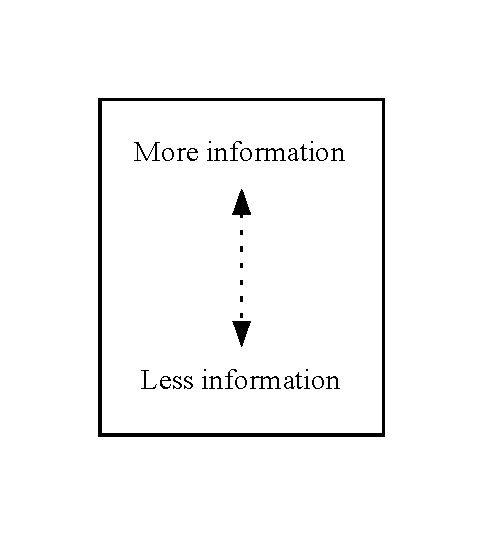
\includegraphics[scale=0.5]{more-information.pdf}
\end{columns}
\end{frame}
}}

\newcommand{\codeslide}[1]{{
\begin{frame}[fragile]
\begin{haskellcode}
#1
\end{haskellcode}
\end{frame}
}}

\newcommand{\imageslide}[2][1]{{
\begin{frame}\begin{center}
\includegraphics[scale=#1]{#2}
\end{center}\end{frame}
}}

\newcommand{\imageslideleft}[2][1]{{
\begin{frame}
\includegraphics[scale=#1]{#2}
\end{frame}
}}

\newcommand{\imagetextslide}[3][1]{{
\begin{frame}\begin{center}

{#3}

\includegraphics[scale=#1]{#2}
\end{center}\end{frame}
}}

\newcommand{\svgslide}[1]{{
\begin{frame}
\begin{center}
\includesvg{diagrams/#1}
\end{center}
\end{frame}
}}

\newcommand{\ctof}{{
\LARGE $\degree F = \degree C \times \frac{9}{5} + 32$
}}

\newcommand{\ftoc}{{
\LARGE $\degree C = (\degree F - 32) \div \frac{9}{5}$
}}

%%----------------------------------------------------------------------------------------
%	TITLE PAGE
%----------------------------------------------------------------------------------------

\title[Propagators]{Propagators: An Introduction} % The short title appears at the bottom of every slide, the full title is only on the title page
\titlegraphic{
\includegraphics[scale=0.2]{data61.eps}}
\author{George Wilson} % Your name
\institute[] % Your institution as it will appear on the bottom of every slide, may be shorthand to save space
{
Data61/CSIRO\\ % Your institution for the title page
\medskip
\href{george.wilson@data61.csiro.au}{george.wilson@data61.csiro.au} % Your email address
}
\date{\today} % Date, can be changed to a custom date

\begin{document}


%%%%%
%%%%% Intro section
%%%%%


\begin{frame}
\titlepage % Print the title page as the first slide
\end{frame}


\begin{frame}

\begin{columns}
  \begin{column}{0.5\textwidth}
    \begin{center}
      
\includegraphics[scale=0.015]{what-are-birds.jpg}

      \nl

      What?
    \end{center}
  \end{column}
  \begin{column}{0.5\textwidth}
    \begin{center}
      
\includegraphics[scale=0.3]{for-what-purpose.jpg}

      \nl

      Why?
    \end{center}
  \end{column}
\end{columns}

\end{frame}


%%%%%
%%%%% History
%%%%%


\begin{frame}

\begin{columns}
\begin{column}{0.5\textwidth}
Beginnings as early as the 1970's at MIT
\begin{itemize}
  \item Guy L. Steele Jr. 
  \item Gerald J. Sussman
  \item Richard Stallman
\end{itemize}

\nl

More recently:
\begin{itemize}
  \item Alexey Radul
\end{itemize}
\end{column}
\begin{column}{0.5\textwidth}

\begin{figure}
\centering
\def\svgwidth{\columnwidth}
\input{circuit.pdf_tex}
\end{figure}

\end{column}
\end{columns}

\end{frame}


\begin{frame}[fragile]

\begin{verbatim}
(define (map f xs)
  (cond ((null? xs) '())
        (else (cons (f (car xs))
                    (map f (cdr xs)))))))
\end{verbatim}
\end{frame}


\begin{frame}
\begin{columns}
\begin{column}{0.005\textwidth}
\end{column}
\begin{column}{0.4\textwidth}
And then
\begin{itemize}
\item Edward Kmett
\end{itemize}
\nl
\nl

\includegraphics[scale=0.2]{haskell.png}
\end{column}
\begin{column}{0.5\textwidth}
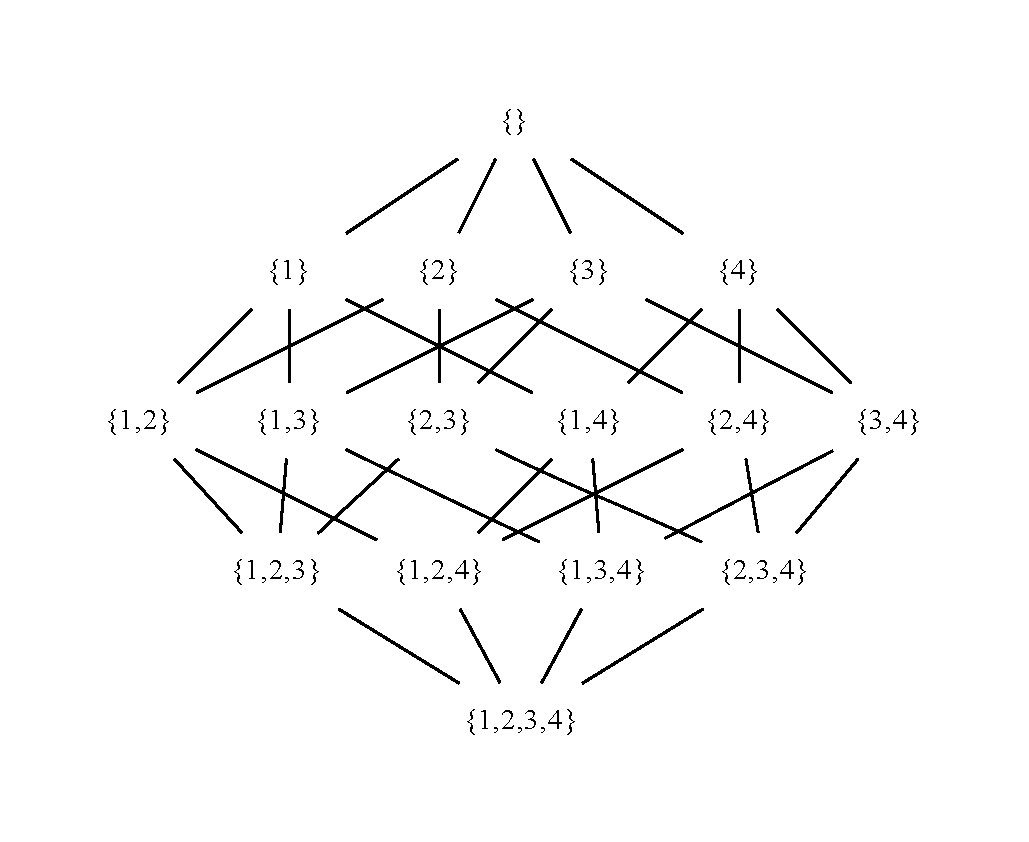
\includegraphics[scale=0.4]{powerset.pdf}

\nl
\nl

{\LARGE
  $x \le y \implies f(x) \le f(y)$
}
\end{column}
\end{columns}
\end{frame}


%%%%%
%%%%% What and why
%%%%%


\begin{frame}

\begin{center}
{\Huge Propagators}
\end{center}

\end{frame}


\begin{frame}
The {\it propagator model} is a model of computation

We model computations as {\it propagator networks}

\pnl

Propagator networks:
\begin{itemize}
\item are extremely expressive
\item lend themselves to parallel and distributed evaluation
\item allow different strategies of problem-solving to seamlessly cooperate
\end{itemize}
\end{frame}


\begin{frame}

A propagator network comprises
\begin{itemize}
\item cells
\item propagators
\item connections between cells and propagators
\end{itemize}

\end{frame}


\imageslide{cell1.pdf}
\imageslide{cell2.pdf}
\imageslide{prop.pdf}

\imageslide{upper1.pdf}
\imageslide{upper2.pdf}
\imageslide{upper3.pdf}

\imageslide{add1.pdf}
\imageslide{add2.pdf}
\imageslide{add3.pdf}
\imageslide{add4.pdf}


%%%%% bidirectionality


\begin{frame}
  \begin{center}
    \begin{LARGE}
      $z \leftarrow x + y$
    \end{LARGE}
  \end{center}
\end{frame}


\begin{frame}
  \begin{center}
    \begin{LARGE}
      $z = x + y$
    \end{LARGE}
  \end{center}
\end{frame}


\begin{frame}
  \begin{center}
    \begin{LARGE}
      $7 = x + 4$
    \end{LARGE}
  \end{center}
\end{frame}


\begin{frame}
  \begin{center}
    \begin{LARGE}
      $7 = 3 + 4$
    \end{LARGE}
  \end{center}
\end{frame}


\begin{frame}
  \begin{center}
    \begin{LARGE}
      $z = x + y$
    \end{LARGE}
  \end{center}
\end{frame}


\begin{frame}
  \begin{center}
    \begin{LARGE}
      $z \leftarrow x + y$

      \nl

      $x \leftarrow z - y$

      \nl

      $y \leftarrow z - x$

    \end{LARGE}
  \end{center}
\end{frame}


\imageslide{badd1.pdf}
\imageslide{badd2.pdf}
\imageslide{badd3.pdf}
\imageslide{badd4.pdf}


\begin{frame}
\begin{center}
{\LARGE Propagators let us express multi-directional relationships!}
\end{center}
\end{frame}

\imagetextslide[0.8]{celsius1.pdf}{\ctof}
\imagetextslide[0.8]{celsius2.pdf}{\ctof}
\imagetextslide[0.8]{celsius3.pdf}{\ctof}
\imagetextslide[0.8]{celsius4.pdf}{\ctof}
\imagetextslide[0.65]{celsius5.pdf}{\ctof \\ \nl \ftoc}
\imagetextslide[0.65]{celsius6.pdf}{\ctof \\ \nl \ftoc}
\imagetextslide[0.65]{celsius7.pdf}{\ctof \\ \nl \ftoc}
\imagetextslide[0.65]{celsius8.pdf}{\ctof \\ \nl \ftoc}
\imagetextslide[0.65]{celsius9.pdf}{\ctof \\ \nl \ftoc}
\imagetextslide[0.65]{celsius10.pdf}{\ctof \\ \nl \ftoc}
\imagetextslide[0.65]{celsius11.pdf}{\ctof \\ \nl \ftoc}
\imageslide[0.65]{celsius12.pdf}
\imageslide[0.65]{celsius13.pdf}
\imageslide[0.65]{celsius14.pdf}
\imageslide[0.65]{celsius15.pdf}
\imageslide[0.65]{celsius16.pdf}


\textslide{
\Large{We can combine networks into larger networks!}
}

\textslide{\Huge{?}}


%%%%% partiality


\textslide{\Large{Cells {\it accumulate information} about a value}}

\imageslide[0.5]{manual/sudoku1.png}
\imageslide[0.5]{manual/sudoku2.png}
\imageslide[0.5]{manual/sudoku3.png}
\imageslide[0.5]{manual/sudoku4.png}
\imageslide[0.5]{manual/sudoku5.png}
\imageslide[0.5]{manual/sudoku6.png}
\imageslide[0.5]{manual/sudoku7.png}
\imageslide[0.5]{manual/sudoku8.png}
\imageslide[0.5]{manual/sudoku9.png}
\imageslide[0.5]{manual/sudoku10.png}
\imageslide[0.5]{manual/sudoku11.png}
\imageslide[0.5]{manual/sudoku12.png}




\textslideleft{

Cells accumulate information in a {\it bounded join-semilattice}

\pnl

A bounded join-semilattice is:

\begin{itemize}
\item A {\it partially ordered set}
\item with a least element
\item such that any set of elements has a {\it least upper bound}
\end{itemize}

\pnl

``Least upper bound'' is denoted as $\vee$ and is usually pronounced ``join''

}

\begin{frame}
\begin{columns}
\column{0.7\textwidth}
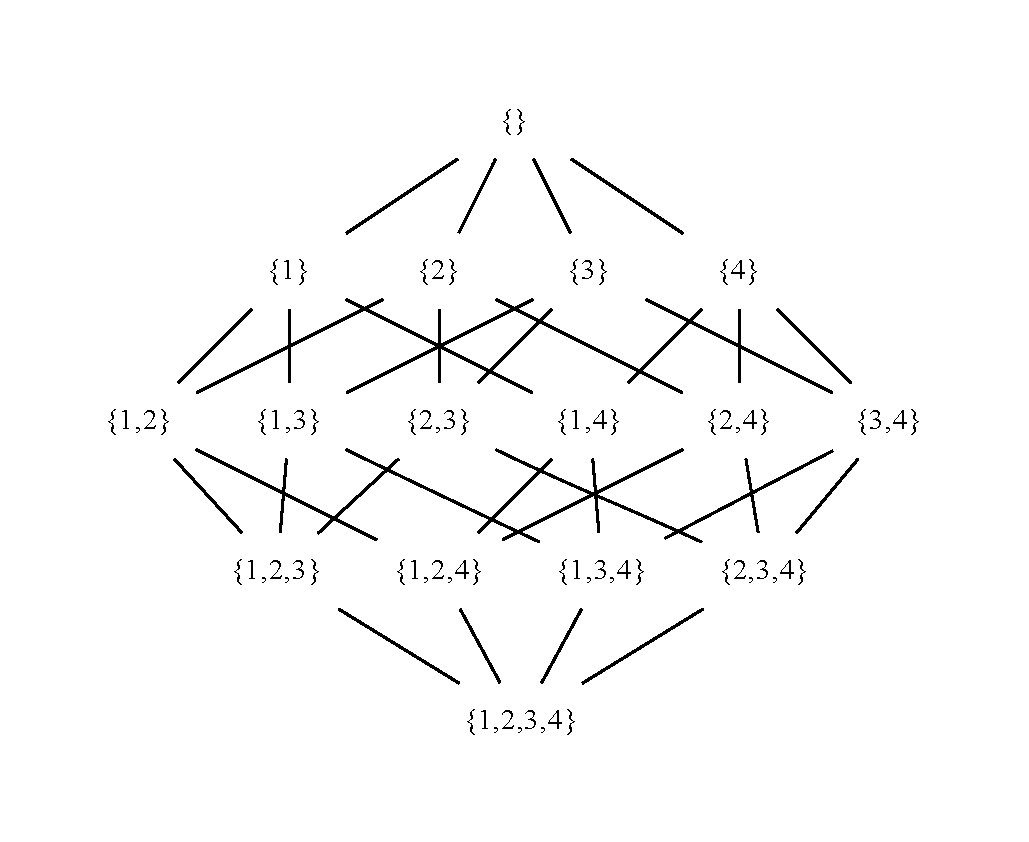
\includegraphics[scale=0.65]{powerset.pdf}
\pause
\column{0.3\textwidth}
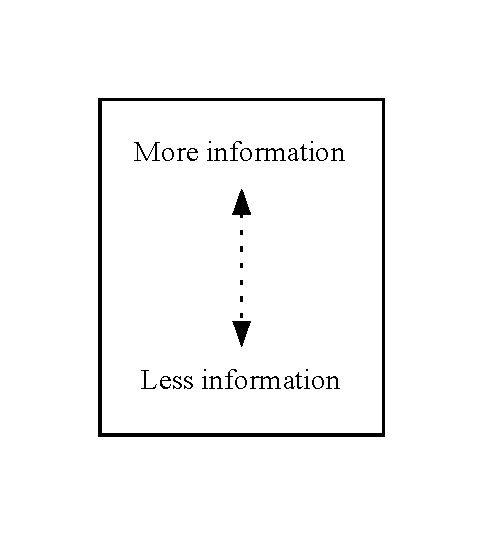
\includegraphics[scale=0.5]{more-information.pdf}
\end{columns}
\end{frame}


\latticeinfoslide{set/powerset-info1.pdf}
\latticeinfoslide{set/powerset-info2.pdf}
\latticeinfoslide{set/powerset-info3.pdf}
\latticeinfoslide{set/powerset-info4.pdf}

\latticeinfoslide{set/powerset1.pdf}
\latticeinfoslide{set/powerset2.pdf}
\latticeinfoslide{set/powerset3.pdf}
\latticeinfoslide{set/powerset4.pdf}
\latticeinfoslide{set/powerset5.pdf}
\latticeinfoslide{set/powerset6.pdf}

\textslideleft{
$\vee$ has useful algebraic properties. It is:

\begin{itemize}
\item A monoid
\item that's commutative
\item and idempotent
\end{itemize}
}

\textslide{
Left identity

$\epsilon \vee x = x$
\nl

Right identity

$x \vee \epsilon = x$
\nl

Associativity

$(x \vee y) \vee z = x \vee (y \vee z)$
\nl

Commutative

$x \vee y = y \vee x$
\nl

Idempotent

$x \vee x = x$
}

\begin{frame}[fragile]
  \begin{haskellcode}
class BoundedJoinSemilattice a where
  bottom :: a
  (\/) :: a -> a -> a
  \end{haskellcode}

  \pnl

  \begin{haskellcode}
data SudokuVal = One | Two | Three | Four
                 deriving (Eq, Ord, Show)
  \end{haskellcode}
  \pause
  \begin{haskellcode}
newtype SudokuSet = S (Set SudokuVal)
  \end{haskellcode}
  \pnl
  \begin{haskellcode}
instance BoundedJoinSemilattice SudokuSet where
  bottom     = S (Set.fromList [One, Two, Three, Four])
  S a \/ S b = S (Set.intersection a b)
  \end{haskellcode}
\end{frame}

\textslideleft{
  We don't write values directly to cells

  Instead we {\it join information in}

  \pnl

  This makes our propagators {\it monotone}, meaning that as the input cells gain information, the output cells gain information (or don't change)

  \pnl

  A function $f : A \rightarrow B$ where $A$ and $B$ are partially ordered sets is {\bf monotone} if and only if, \\
  for all $x,y \in A .$ $x \leq y \implies f(x) \leq f(y)$
}

\textslide{
  All our lattices so far have been fininte

  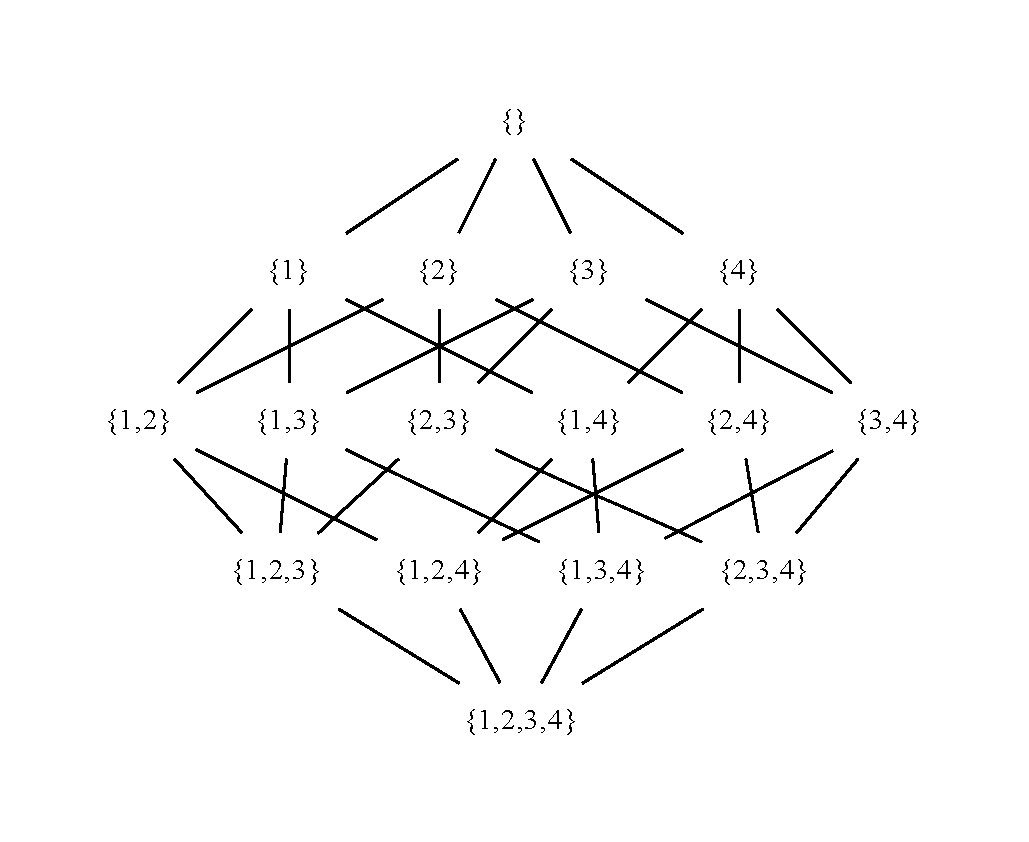
\includegraphics[scale=0.6]{powerset.pdf}
}

\textslideleft{
  The bounded join-semilattice laws combined with the finiteness of our lattices, \\
  make propagator networks deterministic, even in the face of parallelism and distribution

  \pnl

  Bounded join-semilattices are already popular in the distributed systems world

  See: Conflict Free Replicated Datatypes

  \pnl

  We can relax these constraints in a few different directions
}

\textslide{
  Our lattices only need the {\it ascending chain condition}

  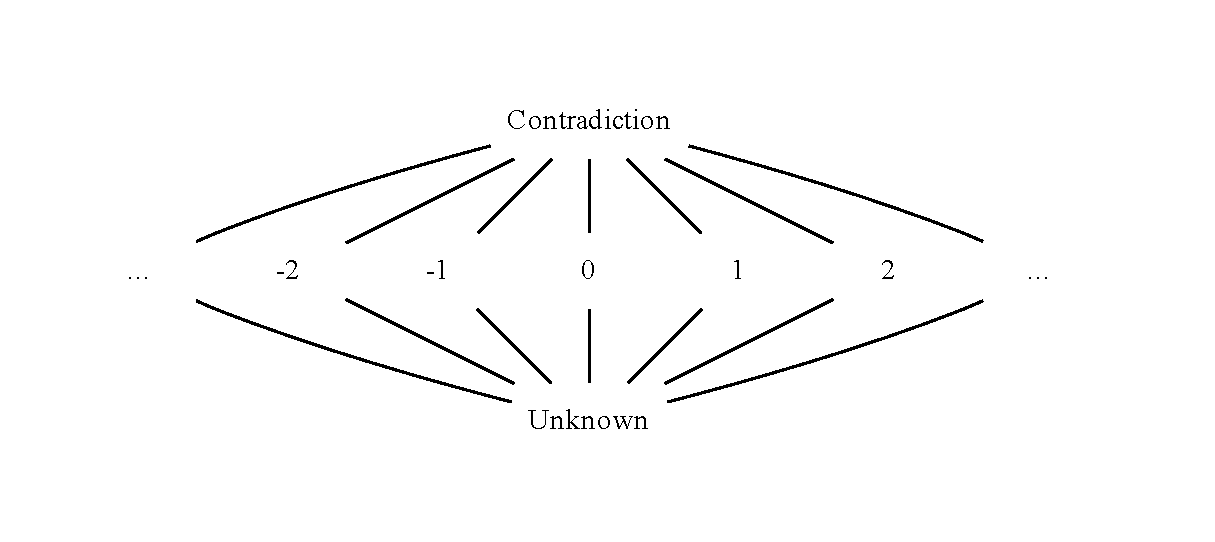
\includegraphics[scale=0.8]{flat.pdf}
}

\textslide{\Huge{?}}

\imageslide{add3.pdf}

%\begin{frame}[fragile]
%\begin{haskellcode}
%data Perhaps a = Unknown | Known a | Contradiction
%\end{haskellcode}
%\end{frame}

\begin{frame}[fragile]

\begin{haskellcode}
data Perhaps a = Unknown | Known a | Contradiction
\end{haskellcode}

\pnl

\begin{haskellcode}
instance Eq a => BoundedJoinSemiLattice (Perhaps a) where

  bottom = Unknown

  (\/) Unknown x           = x
  (\/) x       Unknown     = x
  (\/) Contradiction _     = Contradiction
  (\/) _     Contradiction = Contradiction
  (\/) (Known a) (Known b) =
    if a == b
      then Known a
      else Contradiction
\end{haskellcode}

\end{frame}

\imageslide{perhaps1.pdf}
\imageslide{perhaps2.pdf}


%\imageslideleft{contradiction4.pdf}
%\imageslideleft{contradiction5.pdf}
%\imageslideleft{contradiction6.pdf}
%\imageslideleft{contradiction7.pdf}
%\imageslideleft{contradiction8.pdf}
%\imageslideleft{contradiction9.pdf}
\imageslide[0.6]{doubleplus0.pdf}
\imageslide[0.6]{doubleplus1.pdf}
\imageslide[0.6]{doubleplus2.pdf}
%\imageslide[0.6]{doubleplus3.pdf}
\imageslide[0.6]{doubleplus4.pdf}
\imageslide[0.6]{doubleplus5.pdf}
\imageslide[0.6]{doubleplus6.pdf}
\imageslide[0.6]{doubleplus7.pdf}
\imageslide[0.6]{doubleplus8.pdf}


\begin{frame}
\begin{columns}
\column{0.5\textwidth}
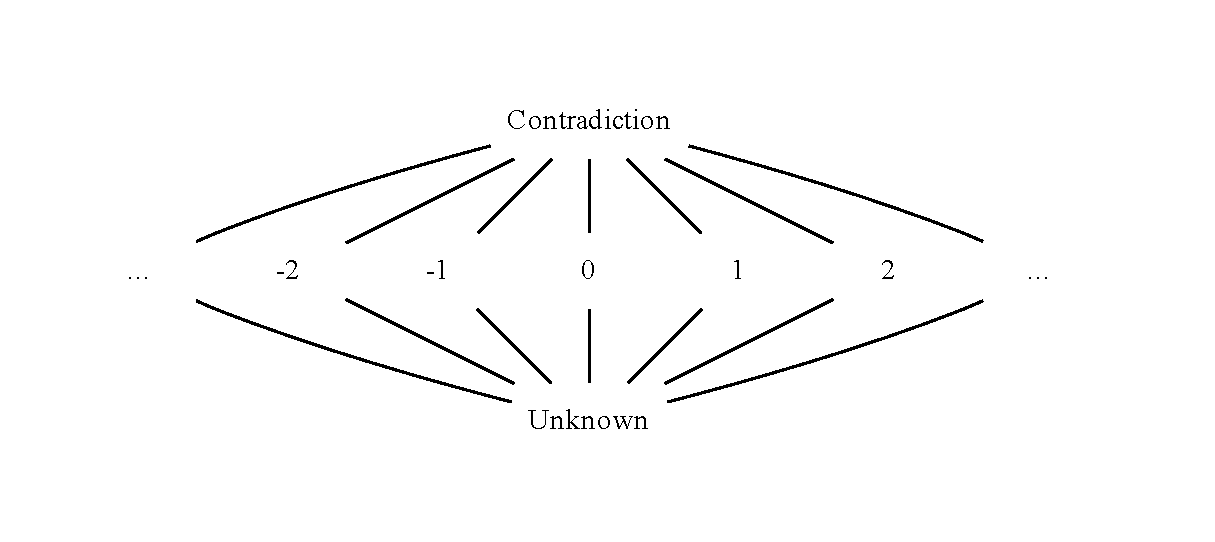
\includegraphics[scale=0.65]{flat.pdf}
\pause
\column{0.2\textwidth}
\column{0.3\textwidth}
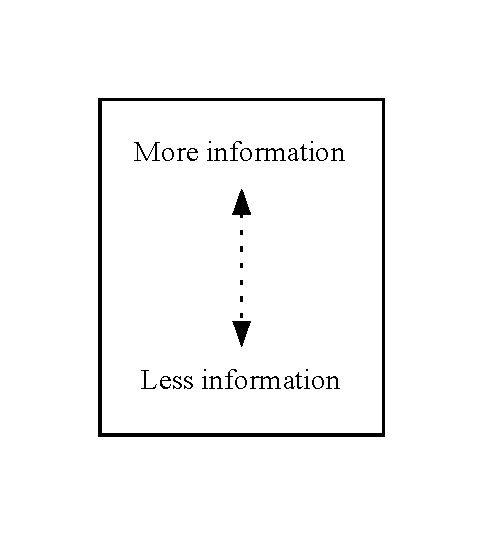
\includegraphics[scale=0.65]{more-information.pdf}
\end{columns}
\end{frame}



\begin{frame}
\begin{center}
\Huge $[1,5]$
\end{center}
\end{frame}


\begin{frame}
\begin{center}
\Huge $[1, 5] \cup [2, 7] = [2,5]$

\pnl

\Huge $[2,5] + [9,10] = [11,15]$
\end{center}
\end{frame}


\imageslide{intervaladd1.pdf}
\imageslide{intervaladd2.pdf}



%\imageslide{manual/screen1.pdf}
\imageslide{manual/screen2.pdf}
\imageslide{manual/screen3.pdf}
\imageslide{manual/screen4.pdf}


\textslide{(Talk about truth-management system machinery)}


%\textslide{{\LARGE
%What types are the values of the cells?
%}}


%\imageslide{cell1.pdf}
%\imageslide{cell2.pdf}
%\imageslide{cell3.pdf}
%\imageslide{cell4.pdf}


%\begin{frame}[fragile]
%\begin{haskellcode}
%data Maybe a = Nothing | Just a
%\end{haskellcode}
%\end{frame}


%\imageslide{maybe1.pdf}
%\imageslide{maybe2.pdf}
%\imageslide{maybe3.pdf}
%\imageslide{maybe4.pdf}

%\imageslide[0.6]{doubleplus3.pdf}

%\imageslideleft{always1.pdf}

%\imageslideleft{always2.pdf}
%\imageslideleft{always3.pdf}
%\imageslideleft{always4.pdf}
%\imageslideleft{contradiction1.pdf}
%\imageslideleft{contradiction2.pdf}
%\imageslideleft{contradiction3.pdf}

%\textslide{
%\LARGE{
%Is this the only type propagator cells can contain?
%
%Will other monoids work?
%}
%
%\pnl
%
%\Large{What about List?}
%}



\begin{frame}

Alexey Radul's work on propagators:

\begin{itemize}
\item Art of the Propagator \\
      \url{http://web.mit.edu/~axch/www/art.pdf}
\item Propagation Networks: A Flexible and Expressive Substrate for Computation \\
      \url{http://web.mit.edu/~axch/www/phd-thesis.pdf}
\end{itemize}
\end{frame}


\textslideleft{

Lindsey Kuper's work on LVars is closely related, and works today:

\begin{itemize}
\item Lattice-Based Data Structures for Deterministic Parallel and Distributed Programming \\
      \url{https://www.cs.indiana.edu/~lkuper/papers/lindsey-kuper-dissertation.pdf}
\item lvish library \\
      \url{https://hackage.haskell.org/package/lvish}
\end{itemize}

}

\textslideleft{
Edward Kmett has worked on:

\begin{itemize}
\item Making propagators go fast
\item Scheduling strategies and garbage collection
\item Relaxing requirements (Eg. not requiring a full join-semilattice, admitting non-monotone functions)
\end{itemize}

Ed's stuff:
\begin{itemize}
\item \url{http://github.com/ekmett/propagators}
\item \url{http://github.com/ekmett/concurrent}
\item Lambda Jam talk (Easy mode): \\
      \url{https://www.youtube.com/watch?v=acZkF6Q2XKs}
\item Boston Haskell talk (Hard mode): \\
      \url{https://www.youtube.com/watch?v=DyPzPeOPgUE}

\end{itemize}
}

\textslideleft{

In conclusion, propagator networks:

\begin{itemize}
\item Admit any Haskell function you can write today \ldots
\item \ldots and more functions!
\item compute bidirectionally
\item give us constraint solving and search
\item parallelise and distribute
\end{itemize}
}

%\textslideleft{
%TODO expand on all this
%
%Things we could build with propagators:
%
%The best spreadsheet
%}


\textslide{\Large{Thanks for listening!}}


\end{document}

